% TODO DRAFT

This project has resulted in a modular peer-to-peer developer library for sending data, encrypted with public key encryption, over a secure connection to another client. The library, \emph{Rymd}, has composed several modules for specific areas such as data storage (section~\ref{sec:datastorage}), cryptography (section~\ref{sec:cryptography}) and communication (section~\ref{sec:p2p}) in order to create a foundation for sending files without central file storage.

For demonstrating the capabilities of Rymd, a sample prototype web application has been created, named \emph{Shuttle}. This front facing client provides a user interface for showing local files, sending files to other users registered in the blockchain, and managing encryption keys. In Shuttle, the user is capable of adding, listing, viewing and deleting files in their local data store, where the files are encrypted and stored along with their metadata. By knowing a recipient's identity, the user is able to share a file with the recipient over an encrypted P2P connection. When sharing a file, the receiving end will instantly show a notification with a remark that the sender wants to share a file. If the recipient chooses to accept the sharing request, the file will download to their local data store.

\begin{figure}[h]
\centering
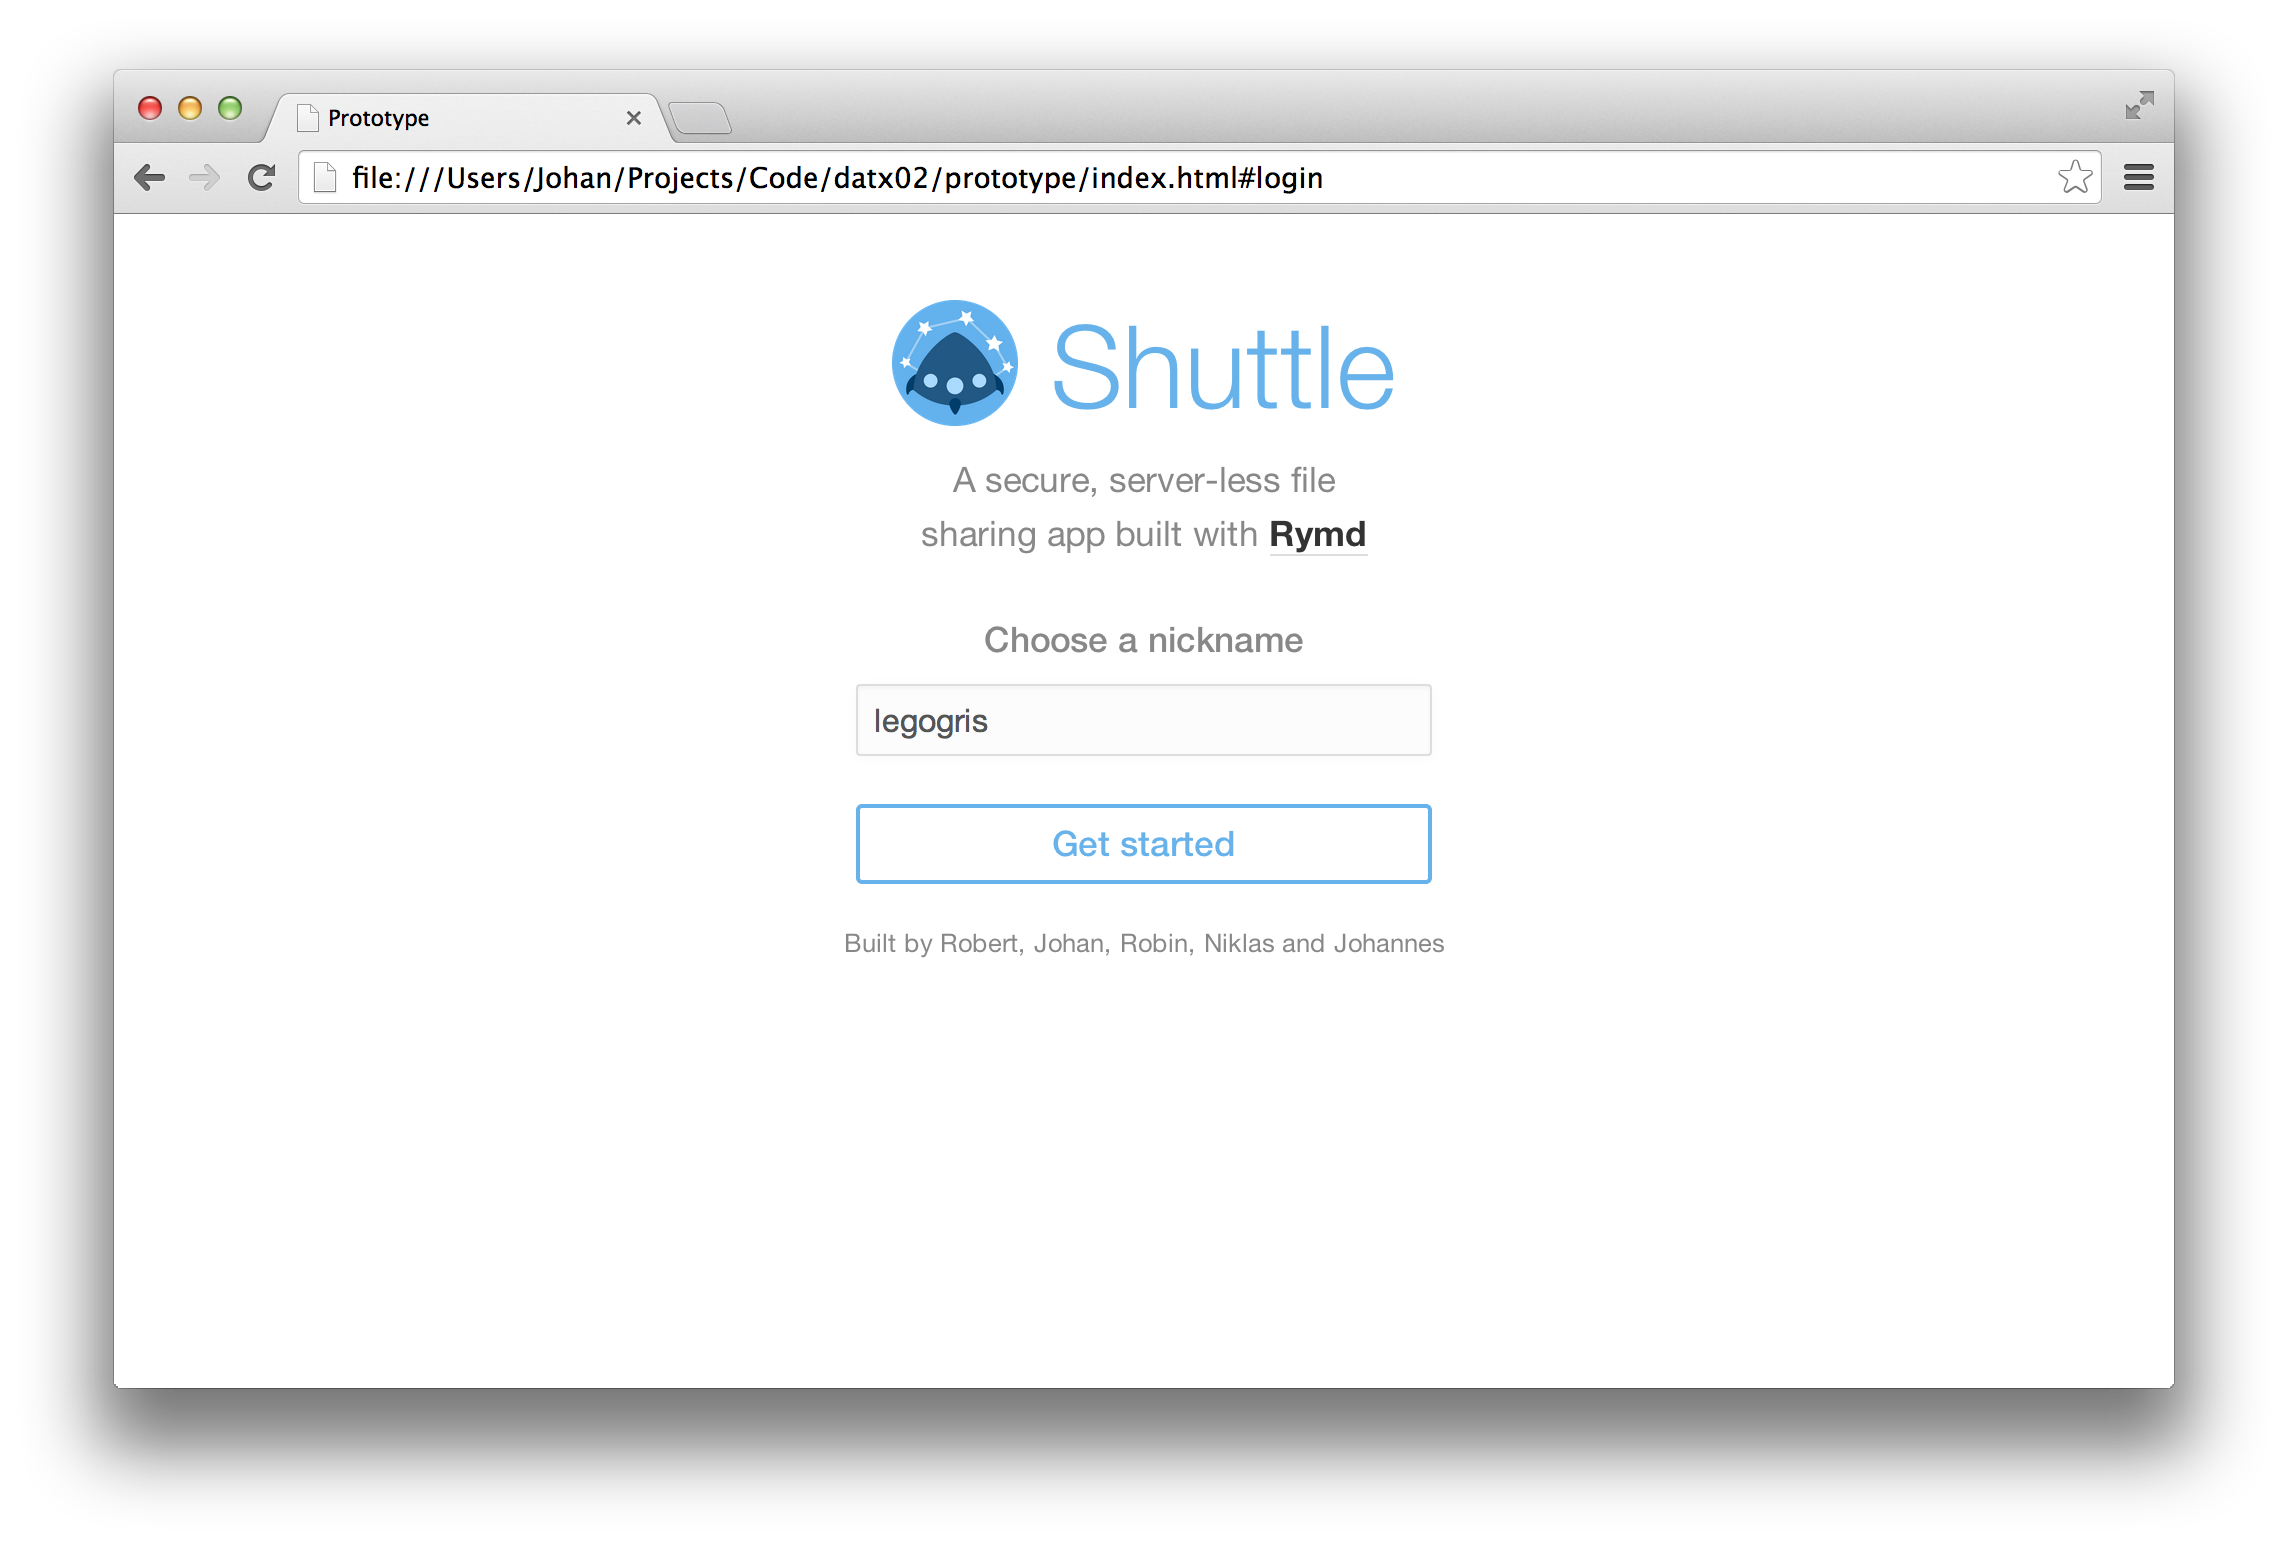
\includegraphics[width=\textwidth,height=0.2\paperheight,keepaspectratio
]{figures/shuttle-login}
\caption{The Shuttle login view}
\label{fig:shuttle-login}
\end{figure}

\begin{figure}[h]
\centering
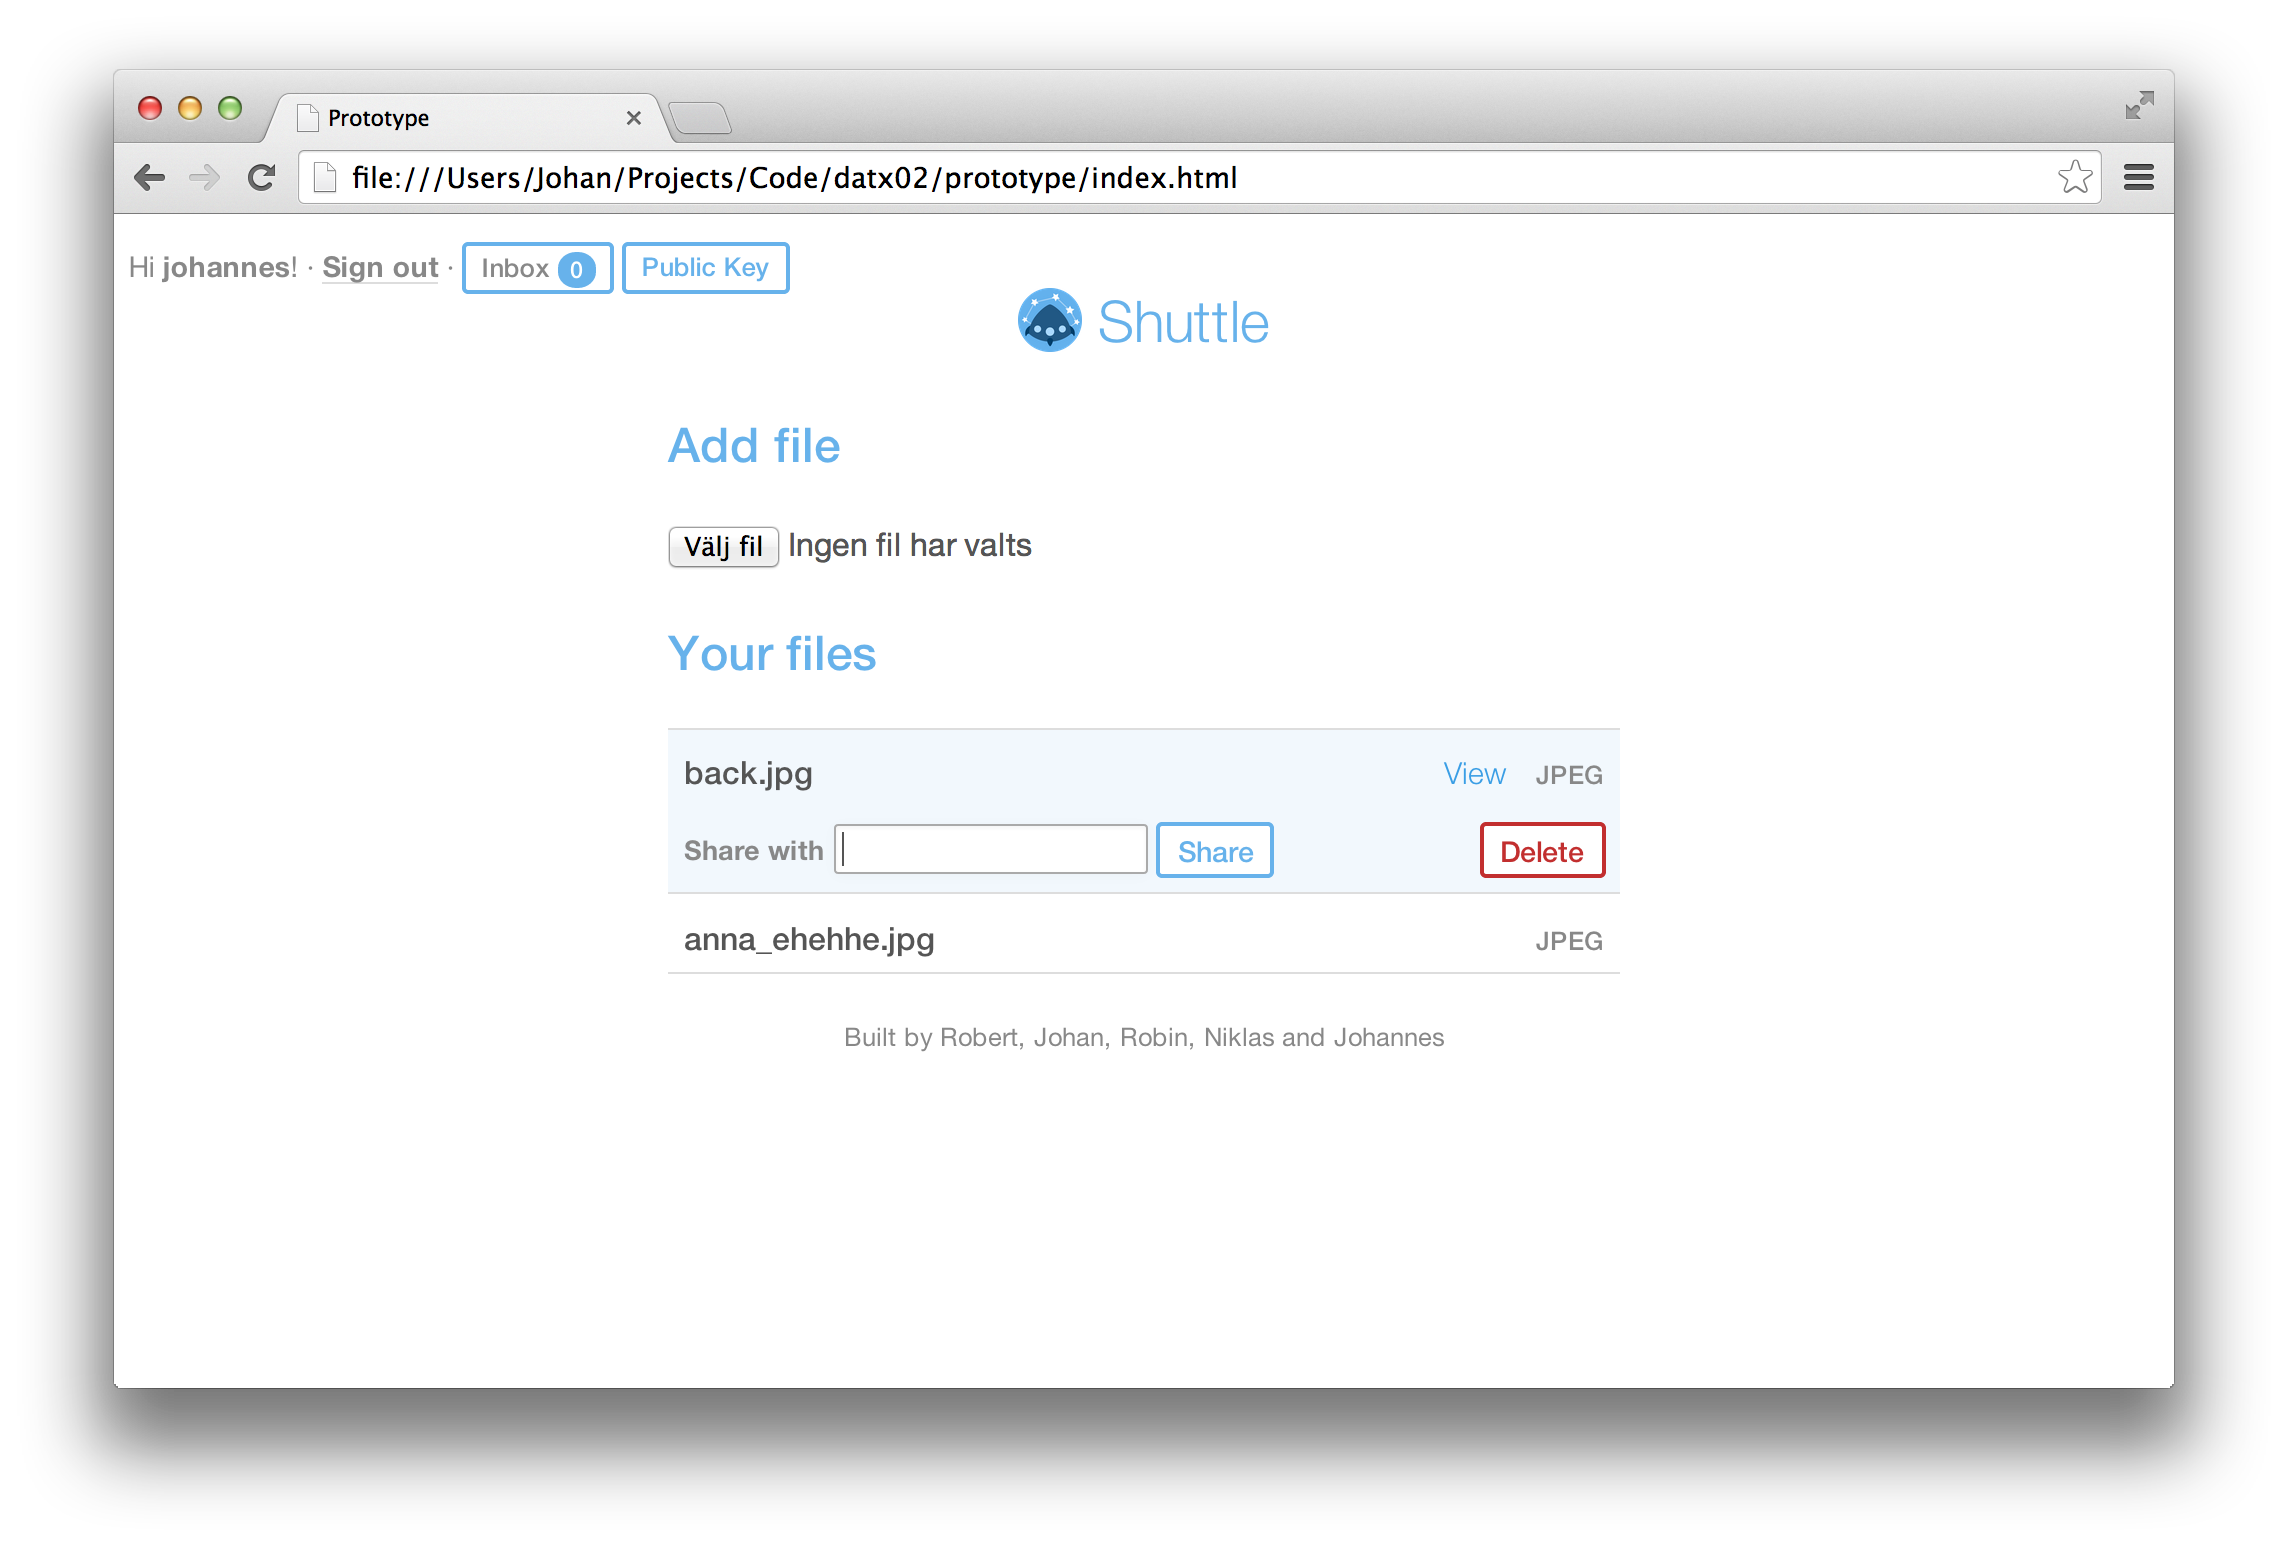
\includegraphics[width=\textwidth,height=0.2\paperheight,keepaspectratio
]{figures/shuttle-files}
\caption{Files listing in Shuttle}
\label{fig:shuttle-files}
\end{figure}

\section{Source code}

Due to the modularity of the system, a number of repositories exist to hold the source code of the different modules. All source code is available at the project's GitHub page: https://github.com/rymdjs. All relevant repositories can be found below:

\begin{description}
  \item[Rymd] https://github.com/rymdjs/rymd
  \item[Shuttle] https://github.com/rymdjs/prototype
  \item[Crypto] https://github.com/rymdjs/crypto. Cryptography module.
  \item[Data Storage] https://github.com/rymdjs/data-storage. IndexedDB adapter.
  \item[PeerJS Connection] https://github.com/rymdjs/peerjs-connection. Connection adapter for PeerJS for doing P2P.
  \item[DHT Client] https://github.com/rymdjs/dht-client. Client module for Namecoin lookups.
  \item[DHT] https://github.com/rymdjs/dht. Node.js HTTP REST adapter for lookups in the Namecoin blockchain.
  \item[Rymd Logger] https://github.com/rymdjs/rymd-logger. Custom debug and flow logger module.
  \item[Rymd Utils] https://github.com/rymdjs/rymd-utils. Globally used utility functions.
\end{description}
